\mysection{Binomial Theorem}

\begin{mysubsection}{}
    We are intereseted in expanding a binomial expression raised to the powewr $n$, $(a+b)^n$, with $n$ being a non-negative integer.

    For the identities we have memorized, we have the following expansion:
    \begin{alignat*}{1}
        (a+b)^0&= 1\\
        (a+b)^1&= a+b\\
        (a+b)^2&= a^2+2ab+b^2\\
        (a+b)^3&= a^3+3a^2b+3ab^2+b^3
    \end{alignat*}
    And for $(a+b)^4$, we can consider $(a+b)^4=(a+b)(a+b)^3$. And inductively, we may consider
    \[(a+b)^n=(a+b)(a+b)^{n-1}.\]
    However, if we find $(a+b)^n$ in such manner, it will be time consuming. Hence we may try to observe a pattern on the coefficient of each terms.
    \begin{figure}[H]
        \centering
        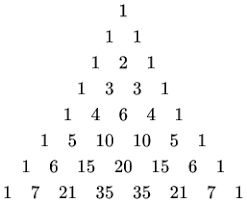
\includegraphics[width=.4\linewidth]{./co3_pic/PascalTriangleNum.png}
    \end{figure}
    If we write the coefficient as a triangle shown above, we may observe some property:
    \begin{enumerate}
        \item The sum of any two adjacent numbers in a row is equal to the immediate number below them.
        \item The first and the last numbers in each row are $1$.
        \item The numbers in each row are symmetrical.
    \end{enumerate}
    The first property can be proved by expanding the expression $(a+b)(a+b)^{n-1}$. The second property can be easily observed that the coefficient of $a^n$ and $b^n$ is $1$.

    Yet, we may as well view it as a combinatorics problem. Take $(a+b)^4$ as an example, if we simply expand it, we will get $16$ terms. And the coefficient we care about are the number of like terms. For example, the coefficient of the term $ab^3$ is the number of times $ab^3$ appear in the expansion. The number of ways to choose one $a$ and three $b$ out of $4$ brackets are ${4\choose 3}$. Same logic apply to other terms. Hence we can get the expansion
    \[(a+b)^4={4\choose 0}a^4+{4\choose 1}a^3b+{4\choose 2}a^2b^2+{4\choose 3}ab^3+{4\choose 4}b^4.\]
    And we can draw the pascal triangle as the form below:
    \begin{figure}[H]
        \centering
        
\includegraphics[width=.5\linewidth]{./co3_pic/PascalTriangleNCR.png}
    \end{figure}
    The symmetric property of the pascal triangle is followed by ${n\choose r}$ equals ${n\choose n-r}$. And with the notation above, we have the binomial theorem:

    \begin{theorem}[thm:]{Binomial Theorem}
        \[(a+b)^n={n\choose 0}a^n+{n\choose 1}a^{n-1}b+{n\choose 2}a^{n-2}b^2+\cdots +{n\choose n-1}ab^{n-1}+{n\choose n}b^n.\]
    \end{theorem}

    And hence the coefficient of the term $a^rb^{n-r}$ is ${n\choose r}$.
\end{mysubsection}

\begin{shortque}[]{1}
    \qitem{%
        Find the coefficient of $x^5$ in the expansion of $(1+2x)^6$.
        }{%
        The $(r+1)$th term is ${6\choose r}(2x)^r={6\choose r}2^rx^r$. Hence coefficient of $x^5={6\choose 5}2^5=192$.
        }{%
        p.1.16
    }

    \qitem{%
        Find the coefficient of the 3rd term in the expansion of $(2+3x)^6$ in ascending powers of $x$.
        }{%
        The $(r+1)$th term is ${6\choose r}2^{6-r}(3x)^r={6\choose r}2^{6-r}3^rx^r$. Hence coefficient of 3rd term, which is when $r=2$, equals ${6\choose 2}2^{6-2}3^2=2160$.
        }{%
        <++>
    }

    \qitem{%
        Find the coefficient of the 4th term in the expansion of $(3x-1)^5$ in descending powers of $x$.
        }{%
        The $(r+1)$th term is ${5\choose r}(3x)^{5-r}(-1)^r={5\choose r}(3x)^{5-r}(-1)^rx^{5-r}$. Hence coefficient of 4th term, which is when $r=3$, equals ${5\choose 3}3^{5-3}(-1)^{3}=-90$.
        }{%
        <++>
    }

    \qitem{%
        Find the constant term in the expansion of $\left(2x-\dfrac{1}{x}\right)^6$.
        }{%
        The $(r+1)$th term is ${6\choose r}(2x)^{6-r}(-\frac{1}{x})^r={6\choose r}2^{6-r}(-1)^rx^{6-2r}$. Hence coefficient of constant term, which is when $6-2r=0$, $r=3$, equals ${6\choose 3}2^{6-3}(-1)^3=-160$.
        }{%
        <++>
    }

    \qitem{%
        The coefficient of the 3rd term in the expansion of $(1+3x)^n$ in ascending powers of $x$ is $252$, where $n$ is a positive integer. Find the value of $n$.
        }{%
        The $(r+1)$th term in the expansion is ${n\choose r}(3x)^r={n\choose r}3^rx^r$.

        When $r=2$, the term is the 3rd term. We have
        \begin{alignat*}{1}
            {n\choose 2}3^2&=252\\
            \frac{n(n-1)}{2}\times 9&=252\\
            n(n-1)&= 56\\
            (n-8)(n+7)&= 0\\
            n&= 8 \textnormal{ or }-7 (\textnormal{rej})
        \end{alignat*}
        }{%
        <++>
    }
\end{shortque}
